\documentclass[12pt]{article}

% --- Paquetes ---
\usepackage[utf8]{inputenc}
\usepackage[T1]{fontenc}
\usepackage[spanish,es-tabla]{babel}
\usepackage[letterpaper, top=3cm, bottom=3cm, left=2.5cm, right=2.5cm]{geometry}
\usepackage{amsmath}
\usepackage{graphicx}
\usepackage[colorlinks=true, allcolors=black]{hyperref}
\usepackage{amssymb} 
\usepackage{fancyhdr}
\usepackage{listings}
\usepackage{xcolor}
\usepackage{titlesec}
\usepackage{booktabs}
\usepackage{enumitem}
\usepackage{float}

% --- Configuración de Encabezado y Pie de Página  fPO(Estilo PDF) ---
\pagestyle{fancy}
\fancyhf{}
\setlength{\headheight}{75pt}

\fancyhead[C]{%
    \begin{minipage}[c]{1.8cm}
        
\includegraphics[width=1.8cm]{imagenes/uta.png}
    \end{minipage}%
    \hfill
    \begin{minipage}[c]{12cm} 
        \centering
        \small {\textbf{UNIVERSIDAD TÉCNICA DE AMBATO}} \\
        \scriptsize FACULTAD DE INGENIERÍA EN SISTEMAS ELECTRÓNICA E INDUSTRIAL \\
        \scriptsize CARRERA DE SOFTWARE \\
        \scriptsize \textbf{CICLO ACADÉMICO: ENERO 2026 -- JULIO 2026}
    \end{minipage}%
    \hfill
    \begin{minipage}[c]{1.8cm}
        \centering
        
\includegraphics[width=1.8cm]{imagenes/fisei.png}
    \end{minipage}%
    \\[0.1cm]
}

\fancyfoot[C]{\thepage}

% --- Configuración de listings para R ---
\definecolor{backcolor}{RGB}{245, 245, 245}
\lstset{
    language=R,
    backgroundcolor=\color{backcolor},
    basicstyle=\ttfamily\small,
    breaklines=true,
    showstringspaces=false,
    frame=single,
    numbers=left,
    numberstyle=\tiny\color{gray},
}

\begin{document}

% --- 4.1.1. Portada ---
\begin{titlepage}
    \centering
    
    \begin{minipage}{0.15\textwidth}
        \centering
        
\includegraphics[width=\textwidth]{imagenes/uta.png}
    \end{minipage}
    \hfill
    \begin{minipage}{0.65\textwidth}
        \centering
        {\large \textbf{UNIVERSIDAD TÉCNICA DE AMBATO} \par}
        {\small Facultad de Ingeniería en Sistemas, Electrónica e Industrial \par}
        {\small Carrera de Software \par}
        \vspace{0.3cm}
        {\small Investigación de Operaciones \par}
    \end{minipage}
    \hfill
    \begin{minipage}{0.15\textwidth}
        \centering
        
\includegraphics[width=\textwidth]{imagenes/fisei.png}
    \end{minipage}

    \vspace{2.5cm}
    
    \hrule
    \vspace{0.4cm}
    {\large \textbf{Optimizaci\'on de Distribuci\'on y Planificaci\'on Temporal en Planta Embotelladora de Agua Purificada} \par}
    \vspace{0.4cm}
    \hrule
    
    \vspace{2.5cm}
    
    {\small Proyecto Académico \par}
    {\small Segundo Parcial \par}
    
    \vspace{2.5cm}
    
    {\centering
    \begin{tabular}{rl}
        \textbf{Estudiantes:} & Añilema Hoffmann Jimmy Alexander \\
                              & Quitto Navarrete Bryan Lenin \\
                              & Rojas Hechavarria Maia Carolina \\
                              & Tisalema Carrillo Patricio Sebastián \\[0.6cm]
        \textbf{Docente:}     & Mat. Inti Becerra, Mg. \\
        \textbf{Fecha:}       & \today \\
        \textbf{Período:}     & Enero 2026 -- Julio 2026 \\
        \textbf{Lugar:}       & Ambato - Ecuador
    \end{tabular} \par}
    
\end{titlepage}

\newpage
\tableofcontents
\newpage

% --- 4.1.2. Resumen (máx. 1 página) ---
\section{Resumen}

\subsection{Problema planteado}
Una planta embotelladora de agua purificada tiene 3 centros de producción y debe abastecer a 4 centros de distribución (CD). Se busca minimizar el costo total de transporte y planificar la instalación de una nueva red de distribución con 7 actividades en un plazo máximo de 40 días.

\subsection{Objetivos del proyecto}
Al completar este proyecto, el estudiante será capaz de:
\begin{enumerate}
    \item Formular un problema de transporte como un modelo de Programación Lineal.
    \item Implementar la solución en R.
    \item Calcular tiempos tempranos, tardíos, holguras y ruta crítica con PERT/CPM.
    \item Interpretar los resultados en términos de costos y tiempos.
    \item Presentar conclusiones ejecutivas con soporte gráfico.
\end{enumerate}

\subsection{Contexto del problema}
Una planta embotelladora de agua purificada tiene \textbf{3 centros de producción} y debe abastecer a \textbf{4 centros de distribución (CD)}. Adicionalmente, debe ejecutar un proyecto de instalación de una nueva red de distribución.

\subsection{Métodos utilizados}
Programación Lineal (Modelo de Transporte) implementado en R (lpSolve) y Gestión de Proyectos mediante técnicas PERT/CPM.

\subsection{Principales resultados numéricos}
[Completar con resultados de la implementación]

\subsection{Conclusión principal}
[Completar según el análisis final]

% --- 4.1.3. Modelo de transporte ---
\section{Modelo de transporte}

\subsection{Descripción del problema}
Se debe determinar cuántos miles de litros enviar desde cada planta a cada CD para minimizar el costo total de transporte, respetando las capacidades de las plantas y las demandas de los CD.

\subsection{Datos proporcionados}
\subsubsection{Capacidad de producción y demanda}
\begin{center}
\begin{tabular}{cc}
    \begin{tabular}{|c|c|}
        \hline
        \textbf{Planta} & \textbf{Capacidad} \\ \hline
        A & 50 \\ \hline
        B & 60 \\ \hline
        C & 40 \\ \hline
    \end{tabular} 
    & 
    \begin{tabular}{|c|c|}
        \hline
        \textbf{CD} & \textbf{Demanda} \\ \hline
        CD1 & 30 \\ \hline
        CD2 & 45 \\ \hline
        CD3 & 35 \\ \hline
        CD4 & 40 \\ \hline
    \end{tabular}
\end{tabular}
\end{center}

\subsubsection{Costos de transporte (\$/miles de litros)}
\begin{center}
\begin{tabular}{|c|c|c|c|c|}
    \hline
    \textbf{Origen \textbackslash Destino} & \textbf{CD1} & \textbf{CD2} & \textbf{CD3} & \textbf{CD4} \\ \hline
    Planta A & 8 & 6 & 10 & 9 \\ \hline
    Planta B & 9 & 12 & 13 & 7 \\ \hline
    Planta C & 14 & 9 & 16 & 5 \\ \hline
\end{tabular}
\end{center}
\subsection{Formulación matemática}
\textbf{Contexto:} Minimizar el costo de envío desde 3 plantas (A, B, C) hacia 4 centros de distribución (CD1, CD2, CD3, CD4) respetando las capacidades de producción y satisfaciendo las demandas.

\begin{itemize}
    \item \textbf{Variables de decisión:} 
    Sea $x_{ij}$ la cantidad de miles de litros enviados desde la planta $i$ al centro de distribución $j$, donde $i \in \{A, B, C\}$ y $j \in \{1, 2, 3, 4\}$.

    \item \textbf{Función Objetivo:}
    Minimizar el costo total de transporte $Z$:
    \begin{equation*}
    \begin{aligned}
    \min Z = & \ 8x_{A1} + 6x_{A2} + 10x_{A3} + 9x_{A4} \\
             & + 9x_{B1} + 12x_{B2} + 13x_{B3} + 7x_{B4} \\
             & + 14x_{C1} + 9x_{C2} + 16x_{C3} + 5x_{C4}
    \end{aligned}
    \end{equation*}

    \item \textbf{Restricciones de oferta (Capacidades de Planta):}
    \begin{align*}
    x_{A1} + x_{A2} + x_{A3} + x_{A4} & \leq 50 \quad \text{(Planta A)} \\
    x_{B1} + x_{B2} + x_{B3} + x_{B4} & \leq 60 \quad \text{(Planta B)} \\
    x_{C1} + x_{C2} + x_{C3} + x_{C4} & \leq 40 \quad \text{(Planta C)}
    \end{align*}

    \item \textbf{Restricciones de demanda (Requerimientos de CD):}
    \begin{align*}
    x_{A1} + x_{B1} + x_{C1} & \geq 30 \quad \text{(CD1)} \\
    x_{A2} + x_{B2} + x_{C2} & \geq 45 \quad \text{(CD2)} \\
    x_{A3} + x_{B3} + x_{C3} & \geq 35 \quad \text{(CD3)} \\
    x_{A4} + x_{B4} + x_{C4} & \geq 40 \quad \text{(CD4)}
    \end{align*}

    \item \textbf{Restricción de no negatividad:}
    \begin{equation*}
    x_{ij} \geq 0 \quad \forall i \in \{A, B, C\}, \forall j \in \{1, 2, 3, 4\}
    \end{equation*}
\end{itemize}\subsection{Tabla de resultados (matriz de envíos)}
[Inserte aquí la matriz de resultados extraída de R]

\subsection{Análisis de sensibilidad}
[Presentar al menos una variación en los datos, por ejemplo: ¿Qué pasaría si la demanda de CD4 aumenta a 50?]

\subsection{Gráfico de flujos}
[Inserte aquí el gráfico representativo de la distribución óptima]

\subsection{Interpretación}
Responda a las siguientes interrogantes basadas en los resultados obtenidos:
\begin{enumerate}
    \item ¿Qué planta envía más producto? ¿Por qué?
    \item ¿Qué ruta es la más utilizada? ¿Qué ruta no se utiliza?
    \item ¿Por qué la Planta C solo envía a un CD?
    \item ¿Qué pasaría si la demanda de CD4 aumenta a 50?
\end{enumerate}

% --- 4.1.4. Gestión del proyecto ---
\section{Gestión del proyecto}

\subsection{Descripción del problema}
La empresa debe ejecutar un proyecto de instalación de una nueva red de distribución con \textbf{7 actividades}. El proyecto debe durar máximo \textbf{40 días hábiles} (8 semanas).

\subsection{Datos proporcionados}
\begin{center}
\begin{tabular}{|c|l|c|c|}
    \hline
    \textbf{Actividad} & \textbf{Descripción} & \textbf{Duración (días)} & \textbf{Predecesor(es)} \\ \hline
    A & Diseño de ruta & 5 & -- \\ \hline
    B & Compra de válvulas & 3 & A \\ \hline
    C & Instalación en CD1 & 4 & B \\ \hline
    D & Instalación en CD2 & 6 & B \\ \hline
    E & Pruebas de flujo & 2 & C, D \\ \hline
    F & Capacitación & 3 & E \\ \hline
    G & Inicio de operación & 1 & F \\ \hline
\end{tabular}
\end{center}

\subsection{Diagrama de red}
[Inserte aquí el diagrama de red mostrando nodos, flechas y relaciones de precedencia]

\subsection{Tabla PERT/CPM}
[Presentar tabla con TE, TL, Holguras y determinación de actividades críticas]

\subsection{Diagrama de Gantt}
[Inserte aquí el diagrama de Gantt con barras de duración, colores para ruta crítica y holguras visibles]

\subsection{Análisis de cumplimiento de plazo}
Responda a los siguientes puntos:
\begin{enumerate}
    \item ¿Cuál es la duración total del proyecto en días?
    \item ¿Cumple con el límite de 40 días? Si no, ¿cuántos días excede?
    \item Si excede, proponga al menos 2 acciones de compresión (crashing).
    \item Si cumple, ¿cuántos días de holgura tiene el proyecto?
\end{enumerate}

% --- 4.1.5. Conclusiones y recomendaciones ---
\section{Conclusiones y recomendaciones}
\begin{itemize}
    \item \textbf{Resumen de hallazgos:} [Resuma los hallazgos del modelo de transporte y tiempos del proyecto]
    \item \textbf{Respuesta a la pregunta:} ¿Se puede ejecutar el proyecto en 8 semanas?
    \item \textbf{Recomendaciones operativas:} [Sugerencias basadas en los resultados obtenidos]
    \item \textbf{Limitaciones del estudio:} [Mencione factores no considerados o restricciones]
\end{itemize}

% --- 4.1.6. Anexos ---
\section{Anexos}
\begin{itemize}
    \item \textbf{Código R completo:}
    \begin{lstlisting}[language=R]
# Inserte aqui el script completo utilizado
# Instalacion de la libreria lpSolve (descomentar la siguiente linea si no esta instalada)
# install.packages("lpSolve")
library(lpSolve)

# 1. Definir la matriz de costos de transporte
costos <- matrix(c(8,  6, 10,  9,
                   9, 12, 13,  7,
                  14,  9, 16,  5), 
                 nrow = 3, byrow = TRUE)

# Asignar nombres a filas y columnas para facilitar la lectura
rownames(costos) <- c("Planta A", "Planta B", "Planta C")
colnames(costos) <- c("CD1", "CD2", "CD3", "CD4")

# 2. Definir las capacidades de oferta (Plantas) y sus signos de restriccion
oferta <- c(50, 60, 40)
signos_oferta <- rep("<=", 3)

# 3. Definir la demanda (Centros de Distribucion) y sus signos de restriccion
demanda <- c(30, 45, 35, 40)
signos_demanda <- rep(">=", 4)

# 4. Resolver el problema usando lp.transport
solucion <- lp.transport(cost.mat = costos, 
                         direction = "min", 
                         row.signs = signos_oferta, 
                         row.rhs = oferta, 
                         col.signs = signos_demanda, 
                         col.rhs = demanda)

# 5. Imprimir los resultados en consola
cat("=== RESULTADOS DEL MODELO DE TRANSPORTE ===\n")
cat("Costo minimo total de transporte: $", solucion$objval, "\n\n")

cat("Matriz de envios optima (en miles de litros):\n")
matriz_resultados <- solucion$solution
rownames(matriz_resultados) <- rownames(costos)
colnames(matriz_resultados) <- colnames(costos)
print(matriz_resultados)
\end{lstlisting}
    \item \textbf{Salidas de consola:} [Capturas o texto de la consola de R]
    \begin{figure}[H]
        \centering
        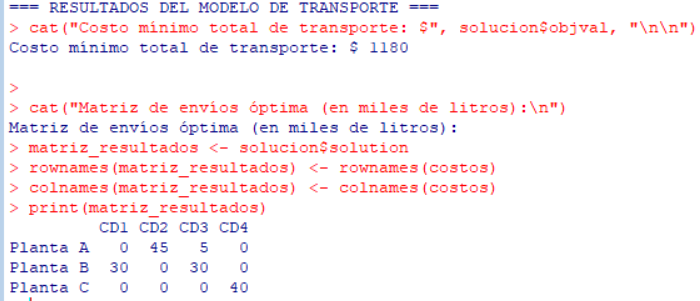
\includegraphics[width=0.75\linewidth]{imagenes/R.png}
        \caption{Resultados en R}
        \label{fig:placeholder}
    \end{figure}
    \item \textbf{Material complementario:} [Gráficos adicionales o tablas de apoyo]
\end{itemize}

\end{document}
